\chapter{Introducción específica} % Main chapter title

\label{Chapter2}

%----------------------------------------------------------------------------------------
%	SECTION 1
%----------------------------------------------------------------------------------------
En el siguiente capitulo se realiza una introducción a las tecnológicas utilizadas en el desarrollo de este trabajo. Estas se aplican a las distintas capas del modelo de arquitectura de IoT (\textit{Internet of Things}).
\section{Protocolos de comunicación}
\label{sec:ejemplo}

Los protocolos de comunicación son estándares que se utilizan para definir la manera en la que se vinculan uno o mas dispositivos. Existe una gran cantidad de protocolos diseñados para resolver distintas problemáticas, a continuación se detallan los utilizados en el desarrollo de este trabajo.

\subsection{SPI \textit{Serial Peripherical Interface}}

EL protocolo de comunicación SPI es un protocolo de comunicación serie, sincrónico y \textit{full duplex}. Los dispositovos sincrónicos cuentan con una señala de clock para la sincronizacioón de los datos enviados y recibidos. A su vez, las señales MOSI \textit{Master Output Slave Input} y MISO \textit{Master Input Slave Output} pemiten la transferencia simultánea de datos entre los dispositivos, esta funcionabilidad recibe el nombre de \textit{full duplex.}

En la figura \ref{fig:SPI} se observa la conexión entre dispositivos SPI.

\begin{figure}[htbp]
	\centering
	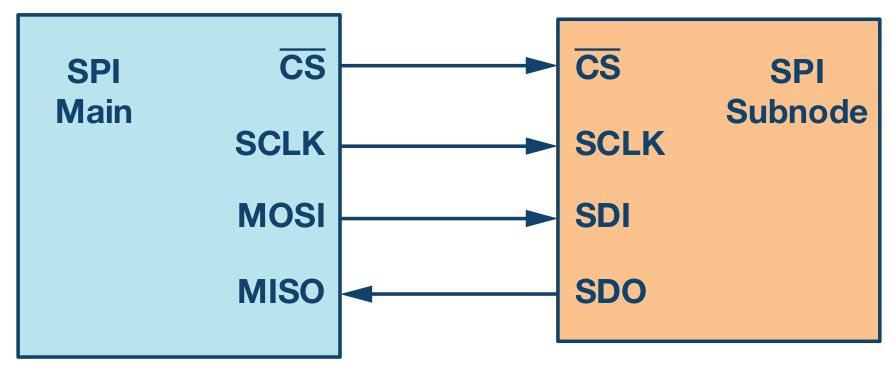
\includegraphics[width=0.6\textwidth]{./Figures/SPI.png}
	\caption{Conexión entre dispositivos SPI maestro - esclavo.}
	\label{fig:SPI}
\end{figure} 

Los dispositivos SPI pueden ser direccionables mediante las señales de CS \textit{chip select} y alcanzar velocidades de reloj de hasta 50MHz. Esto permite una gran capacidad de transferencia de datos, motivo por el cual son utilizados en dispositivos como, pantallas LCD, módulos ethernet y memorias entre otros. 


\subsection{I2C \textit{Inter Integrated Circuit}}

I2C es un protocolo de comunicación serie, sincrónico y bidireccional con un número reducido de hilos para su conexión. Se caracteriza por ser muy versátil y económico, el protocolo I2C se ha implementado en mas de 1000 circuitos integrados que han sido fabricados por mas de 50 compañías. Además, se utiliza en arquitecuras de control como SMBus   \textit{System Management Bus}, DDC    \textit{PMBus Power Management Bus}, IPMI   \textit{Intelligent Platform Management Interface}, DDC   \textit{Display Data Channel} and ATCA   \textit{Advanced Telecom Computing Architecture}.

Cada dispositivo cuenta con una dirección única e inalterable para su direccionamiento. De acuerdo al tipo, pueden incorporar una o mas entradas CS \textit{chip select} para comunicarse con dispositivos idénticos sobre el mismo bus.

En la figura \ref{fig:I2C} se observa el conexionado de dispositivos en un bus I2C.

\begin{figure}[htbp]
	\centering
	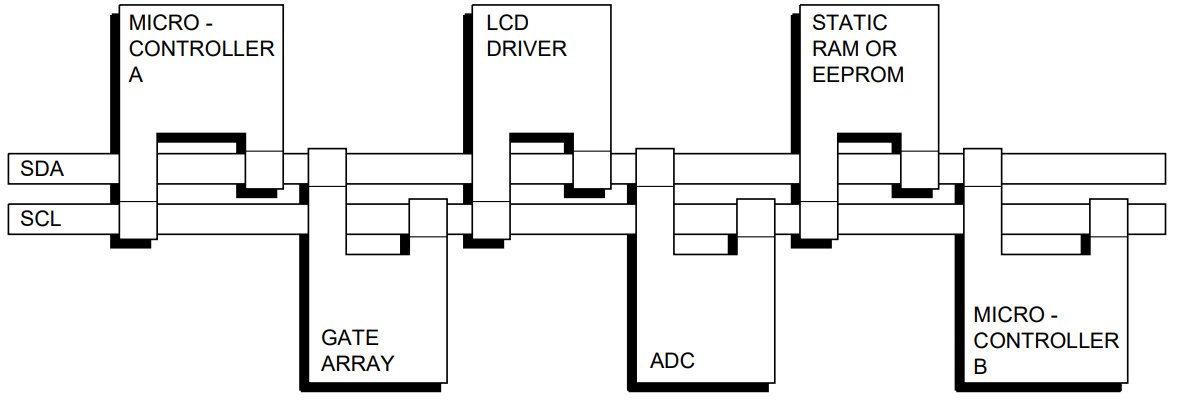
\includegraphics[width=0.8\textwidth]{./Figures/I2C.png}
	\caption{Bus de conexión de dispositivos I2C.}
	\label{fig:I2C}
\end{figure} 

Las velocidades de comunicación varían desde los 100 kHz a los 5MHz, en la actualidad cuentan con dispositivos para aplicaciones, militares, medicinales e industriales. Entre los más utilizados se pueden encontrar, memorias, conversores ADC, DAC, sensores de temperatura y humedad, RTC \textit{Real Time Clock}, giróscopos y otros.

%\subsection{UART \textit{Universal Asincronous Receiver Transmitter}}
%
%El protocolo de comunicación UART es uno de los más antiguos y utilizados para comunicaciones serie. Se caracteria por ser asincrónico y no direccionable limitando su aplicación a enlaces punto a punto.
%
%
%Este protocolo es asincrónico, por lo que no cuenta una señal de clock, esta característica reduce la cantidad de hilos de conexión como se detalla en la Figura \ref{fig:UART}
%
%
%\begin{figure}[htbp]
%	\centering
%	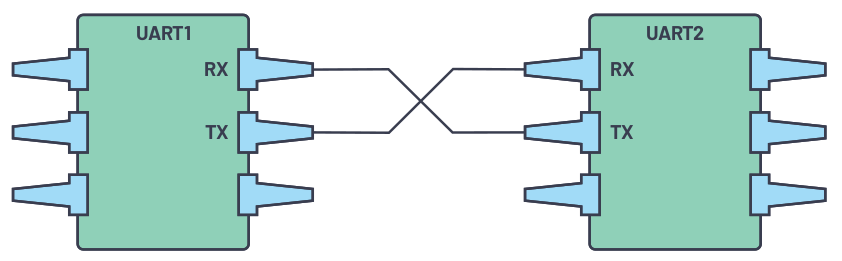
\includegraphics[width=0.6\textwidth]{./Figures/UART.png}
%	\caption{Conexión entre dispositivos UART.\protect\footnotemark.}
%	\label{fig:UART}
%\end{figure} 
%
%A diferencias de los protocolos I2C y  SPI, su velocidad de comunicación es muy inferior. Dedido a su sencillez y bajo costo, se continúa utilizando en algunos dispositivos como, módulos WiFi, módulos LoRa, interfaz de comunicación a PC e impresoras.
%
%\subsection{LoRa \textit{Long Range}}
%
%LoRa es una tecnología de comunicación inalámbrica que utiliza la modulación CSS(\textit{Chip Spread Spectrum}) desarrollada por la empresa Semtech. 
%La utilización de este tipo de modulación posee grandes ventajas de alcance, inmunidad al ruido y consumo.
%En la figura \ref{fig:LoRa} se observa la forma de onda modulada de un dispositivo LoRa. 
%
%\begin{figure}[htbp]
%	\centering
%	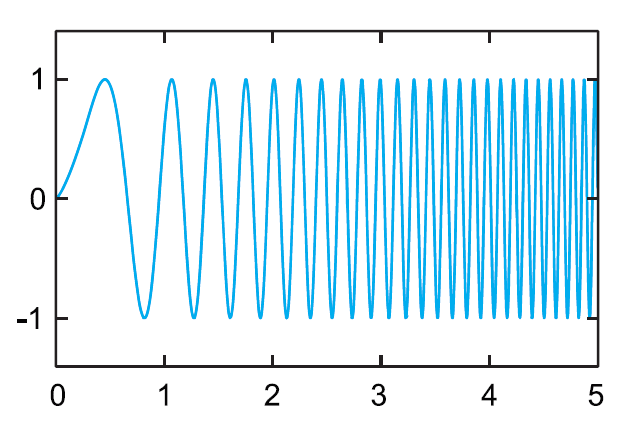
\includegraphics[width=0.3\textwidth]{./Figures/LoRa.png}
%	\caption{Modulación CSS.\protect\footnotemark.}
%	\label{fig:LoRa}
%\end{figure} 
%
%Los dispositivos LoRa utilizan el espectro de frecuencias no licenciado ISM ( \textit{Industrial, Scientific and Medical}) de 915 MHz para el caso de nuestro país, esto reduce el costo operativo de la instalación de dispositivos con esta tecnología.
%
%Con la incorporación del \textit{stack} LoRaWAN, esta tecnología se ha convertido en una de las mas populares del ecosistema IoT.
%
%
%\subsection{ModBUS TCP}
%
%Modbus es un protocolo de aplicación abierto Maestro/Esclavo que se puede utilizar en distintas capas físicas. 
%Modbus TCP significa que el protocolo Modbus se utiliza en la parte superior de Ethernet TCP/IP, un protocolo orientado a la conexión con el que se busca asegurar la entrega de datos. En la figura \ref{fig:ModBUS} puede observarse una arquitectura típica ModBUS.
%
%\begin{figure}[htbp]
%	\centering
%	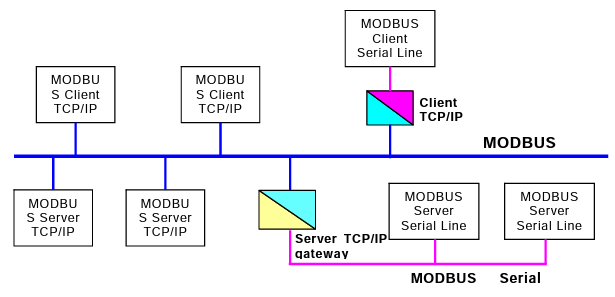
\includegraphics[width=0.7\textwidth]{./Figures/ModBUS.png}
%	\caption{Arquitectura de comunicación ModBUS TCP.\protect\footnotemark.}
%	\label{fig:ModBUS}
%\end{figure} 
%
%Este protocolo ha sido adoptado en la industria por una gran cantidad de fabricantes y en dispositivos controladores lógicos programables, interfase hombre máquina, sensores, actuadores, variadores de velocidad, etc.
%
%ModBUS es un protocolo sencillo, económico y de rápida implementación. Dada su integración existente en los distintos componentes industriales, es muy utilizado cuando se requiere obtener datos de dispositivos industriales. 
%
%\subsection{HTTP \textit{Hypertext Transfer Protocol}}
%
%HTTP es un protocolo de la capa de aplicación para la transmisión de documentos hipermedia, como HTML \textit{HyperText Markup Language}. 
%
%Es un protocolo del tipo cliente - servidor, en el que un cliente establece una conexión con el servidor, realiza una petición y espera hasta que recibe una respuesta. 
%
%Las peticiones se realizan mediante métodos, entre los más utilizados se pueden encontrar, el método PUT, GET, UPDATE Y DELETE. 
%
%En la figura \ref{fig:HTTP} se detalla la acción de cada uno de los métodos mencionados.
%
%\begin{figure}[htbp]
%	\centering
%	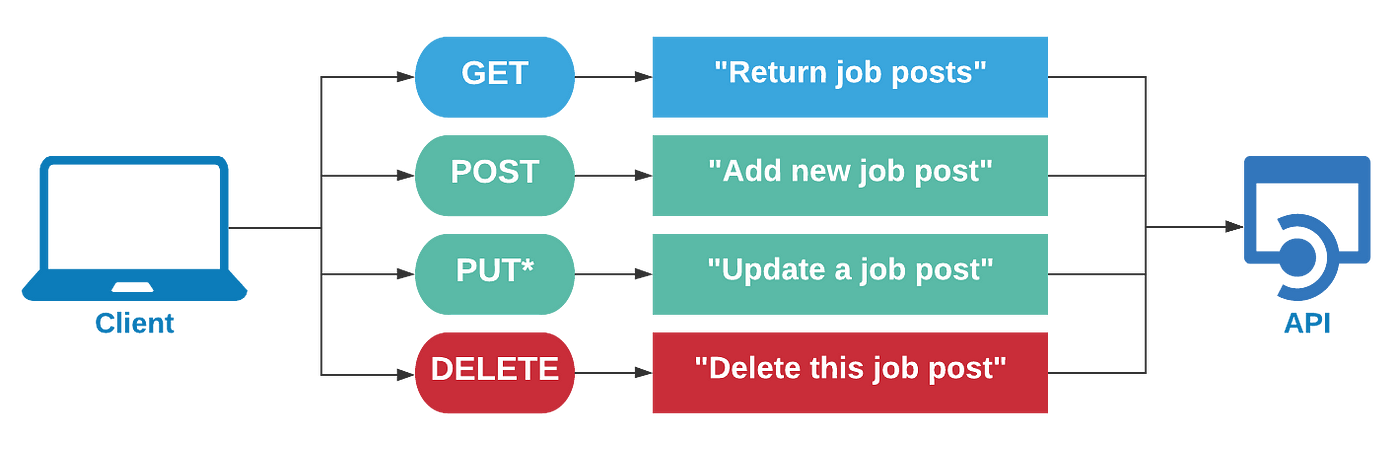
\includegraphics[width=0.6\textwidth]{./Figures/HTTP.png}
%	\caption{Métodos HTTP de uso frecuente.\protect\footnotemark.}
%	\label{fig:HTTP}
%\end{figure} 
%
%%https://miro.medium.com/v2/resize:fit:1400/1*wpbYhweLr38h8fUnuFT0Fg.png
%%https://developer.mozilla.org/es/docs/Web/HTTP
%
%El manejo de datos se encuentra prácticamente cubierto con la utilización de estos cuatro métodos.
%
%En materia de seguridad, el protocolo http puede encriptarse sobre TLS \textit{Transport Layer Security} o bien sobre SSL \textit{Secure Sockets Layer}.
%
%\subsection{Wi-Fi}
%
%La tecnología de red Wi-Fi \textit{Wireless Fidelity} es un protocolo de red inalámbrico basado en las normas IEEE 802.11. 
%
%Las normas IEEE 802.11 especifican los protocolos de capa física y control de acceso al medio para la implementación de una red de área local que permita la comunicación entre dispositivos. 
%
%La evolución de la tecnología Wi-Fi viene dada por la actualización permanente de las normas IEEE 802.11 en repuesta a las necesidades de conectividad que se demandan.
%
%En la figura \ref{fig:WIFIEVO} se observa la evolución de la tecnología Wi-Fi.
%
%%https://softwarelab.org/es/blog/que-es-wi-fi/
%%https://en.wikipedia.org/wiki/IEEE_802.11
%%https://techunwrapped.com/know-the-characteristics-and-speed-of-the-new-wifi-7-or-802-11be/
%
%\begin{figure}[htbp]
%	\centering
%	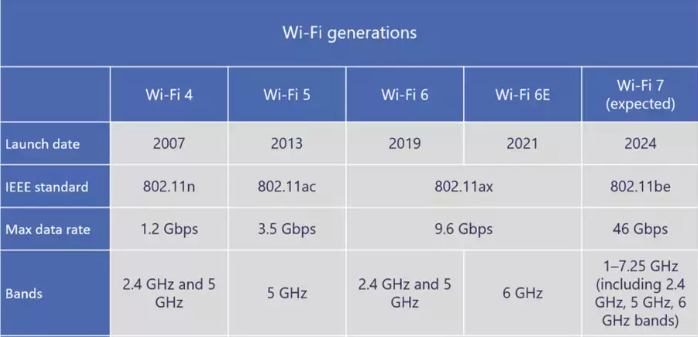
\includegraphics[width=0.7\textwidth]{./Figures/WIFIEVO.png}
%	\caption{Evolución de la tecnología Wi-Fi.\protect\footnotemark.}
%	\label{fig:WIFIEVO}
%\end{figure} 
%
%En la actualidad, la tecnología Wi-Fi se encuentra disponible en un gran número de dispositivos hogareños, industriales y \textit{weareables}.
%
%\subsection{MQTT}
%
%
%
%\section{Tecnologías de backend}
%
%
%
%\section{Tecnologías de frontend} 
%
%
%
%\section{Dispositivos Bare Metal}
%
%
%
%\section{Herramientas utilizadas}
